\chapter{Análsis del problema}
\label{chap:analisis-problema}

\section{Seguridad en la autenticación}

La autenticación del usuario es el punto de entrada a diferentes redes o instalaciones informáticas en las que se presta un 
conjunto de servicios a los usuarios o se puede realizar un conjunto de tareas. 

Una vez autenticado, el usuario puede acceder, por ejemplo a la Intranet de una empresa, a consolas, bases de datos, edificios 
vehículos, etc. La usabilidad de los mecanismos de autenticación se investiga cada vez con más detenimiento y dado que los 
estos son concebidos, implementados, puestos en práctica y corrompidos por teceras personas, hay que tener en cuenta los factores 
humanos en su diseño. 

Actualmente existen múltiples métodos para autenticar a un usuario contra un sistema, siendo el más común es el par de claves 
usuario y contraseña, pero no es el único. El uso de certificados está cada vez más extendido en Infraestructuras de Clave 
Pública (\acf[first-style=short]{pki}). 

Para garantizar que un sistema es necesario que se garantizen tres aspectos \cite{bases_seguridad}:

\begin{itemize}
    \item \textit{Confidencialidad}: prevenir la divulgación no autorizada de la información
    \item \textit{Integridad}: prevenir modificaciones no autorizadas de la información
    \item \textit{Disponibilidad}: prevenir interrupciones no autorizadas de los recursos informáticos
\end{itemize}

Usar un método de autenticación no implica que el sistema sea completamente seguro. De echo, la autenticación se convierte en 
un proceso más robusto y fiable aplicando múltiples métodos, también llamado \acf[first-style=short]{mfa}. Este mecanismo propone tres tipos 
de factores que permiten a un usuario vincularlo con las credenciales establecidas \cite{ometov2018multi}:

\begin{enumerate}
    \item \textit{Factor conocimiento}: algo que el usuario conoce (contraseña)
    \item \textit{Factor pertenencia}: algo que el usuario tiene (token)
    \item \textit{Factor biometrico}: algo que el usuario es (huella dactilar) 
\end{enumerate}

La autenticación basada en múltiples factores provee un nivel de seguridad elevado y facilita una protección continua de 
dispositivos y otros servicios críticos ante accesos no autorizados usando dos o más factores.

Además de la robustez de la seguridad durante el proceso de autenticación, la usabilidad se convierte a su vez en una cuestión 
estratégica en el establecimiento de métodos de autenticación de  usuarios.

La usabilidad puede definirse como ``la medida en que un producto puede ser utilizado por determinados usuarios para alcanzar 
determinados objetivos con eficacia, eficiencia y satisfacción en un contexto de uso específico''. La usabilidad de la seguridad se 
ocupa del estudio de cómo debe tratarse la información de seguridad en la interfaz de usuario y de cómo deben ser los mecanismos 
de seguridad y los sistemas de autenticación deben ser fáciles de usar \cite{braz2006security}.

Este sistema \cite{multipauthpaper} propone un mecanismo de autenticación usable, de múltiples factores y escalable gracias 
principalmente al uso de dispositivos electrónicos con circuitos integrados como es Arduino así como del protocolo MQTT.

\subsection{Seguridad en IoT}

El Internet de las cosas (\acf[first-style=short]{iot}) es un término relativamente nuevo. Se puede definir como una red abierta y completa de 
objetos inteligentes que tienen la capacidad de auto-organizarse, compartir información, datos y recursos, reaccionar y actuar 
ante situaciones y cambios en el entorno \cite{madakam2015internet}. 

El IoT ha facilitado la interconectividad entre dispositivos ayudando a conectar sensores, vehículos, hospitles, industrias y 
consumidores a través de Internet. Las arquitecturas en IoT son cada vez más complejas, descentralizadas y fluidas dado el 
incremento de dispositivos que se comunuican entre sí y es por ello que la seguridad juega un papel fundamental en él. 
Los dispositivos IoT deben ser seguros y no pueden ser manipulados por terceras personas no autorizadas. 

\subsection{\acf[first-style=short]{mqtt}}

Es un protocolo de comunicación que funciona a nivel de la capa de aplicación. Es usado principalmente en entornos
con dispositivos IoT por ser un protocolo con un consumo de bando de ancha y batería mínimo \cite{sugumar2020mqtt}.

A diferencia del protoclo de comunicación \acf[first-style=short]{http} que funciona mediante petición-respuesta, MQTT está basado es 
publicación-respuesta. Este modelo de protocolo requiere de un broker mensajero. Existen múltiples tipos de brokers como 
Mosquitto \cite{eclipse_2018}, HiveMqtt \cite{hivemq}, Mosca \cite{moscajsmosca_2021}, cloudMQTT \cite{cloudmqtt}, MQTT.Js 
\cite{mqttjs}, etc. Para el trabajo propuesto, se usa Mosquitto.

\subsubsection{Funcionamiento del protocolo MQTT}

El cliente MQTT se conecta el broker MQTT subscribiéndose a un tópico. Un tópico es un identificador al cual los nodos se subscriben
y por el que publican mensajes. Si algun mensaje es publicado por un tópico, este llega a todos los nodos que estés suscritos al 
mismo. Se representa con una cadena de caracteres separada por el símbolo $/$ indicando el elemento, dentro de una jerarquía, al 
que se subscribe. 
Un ejemplo de un tópico sería $cocina/sensor1/temperatura$ de tal forma que el cliente obtiene la información de temperatura que 
le llega el sensor1 en la cocina. MQTT se basa en el protoclo TCP/IP para la transmisión de datos. 
El cliente siempre interactua con el broker. No obstante, puede haber múltiples brokers que intercambien datos segun los 
tópicos de subscripción.

\subsubsection{Seguridad en MQTT}
Para garantizar un nivel de seguridad elevado en cuanto a la transmisión de datos se refiere, este protocolo usa por encima
TLS para garantizarlo. Este protolo crea un canal seguro entre el cliente y el broker, parecido a como funciona en los 
navegadores web. Para ello es necesario un certificado del servidor de confianza. 

\subsubsection{Ventajas de MQTT sobre HTTP}

En HTTPS, no se mantiene una conexión continua. El cliente tiene que mandar petición de sondeo (\textit{poll request}) donde 
este solicita información al servidor acerca de la nueva petición de conexión TCP así como la negociación del tipo de 
encriptación SSL/TLS. 

A diferencia de HTTPS, MQTT establece una única conexión inicial. MQTT mantiene un flujo de mensajes fijo (\textit{keep alive})
entre aplicaciones sobre la conexión TCP de tal forma que las aplicaciones pueden detectar cuando una conexión está rota.

\subsection{Criptografía de Curva Elíptica}

La Criptografía de Curva Elíptica (\acf[first-style=short]{ecc}) pertenece a las tres familias de algoritmos de clave pública de gran relevancia 
(factorización de enteros, logaritmos discretos y curva elíptica). Este último nació entorno a mitad de los años 80.
ECC provee del mismo nivel de seguridad que \acf[first-style=short]{rsa} o sistemas logarítmicos discretos con operaciones considerablemente 
pequeñas. ECC está basado en el problema de logaritmo discreto (\acf[first-style=short]{dlp}) \cite{mccurley1990discrete}. ECC tiene beneficios 
en cuanto a su capacidad computacional ya que requiere de menos operaciones computacionales y tiene un consumo de ancho de banda 
muy inferior debido a la pequeña longitud de las claves y firmas con respecto otros como RSA. Esto lo hace ídoneo en arquitecturas
que intervienen dispositivos electrónicos de bajo consumo (Arduinos, Raspberry Pi, etc). No obstante, las operaciones RSA que 
implican una clave pública más pequeña son más rápidas que ECC.

El objetivo de esta sección es explicar las bases de este algoritmo sin entrar en detalles matemáticos. Para mayor documentación
se sugiere leer el libro \cite{paar2009understanding} del cual se ha sacado la información.

Esta sección se distribuye de la siguiente manera: definición del concepto de curva elíptica, problema de logaritmo discreto 
aplicado a las curvas elípticas, algoritmo ECDSA y comparativa con RSA.

\subsubsection{Definición de curva elíptica}

De las ecuaciones polinómicas de una circunferencia y una elipse se pueden sacar diferentes tipos de curvas. Las curva elíptica
es un tipo especial de ecuación polinómica. En criptografía se trabaja sobre un conjunto de números finitos, más popularmente
campos primo, donde todas las operaciones aritméticas se desarrollan sobre módulo \textit{p}, siendo este un número primo.

La definición de curva elíptica es la siguiente:

\begin{definition}[Curva Elíptica]
    La curva elíptica sobre $\mathbb{Z}_{p}$, $\textit{p} > 3$, es el conjunto de pares de punto $\textit{(x,y)} \in \mathbb{Z}_{p}$ 
    que cumplen 
    \begin{equation}
        y^2 = x^3 + ax + b \; mod \; p
    \end{equation}
    junto a un punto infinito imaginario \textit{O}, donde 
    \begin{equation}
        a, b \in \mathbb{Z}_{p}
    \end{equation} 
    y la condición
    \begin{equation}
        4a^3 + 27b^2 \not = 0 \; mod \; p
    \end{equation}
\end{definition}

Ejemplo de una curva elíptica:

\begin{figure}[H]
    \centering
    \begin{tikzpicture}
        \begin{axis}[
                xmin=-2,
                xmax=4,
                ymin=-7,
                ymax=7,
                xlabel={$x$},
                ylabel={$y$},
                scale only axis,
                axis lines=middle,
                % set the minimum value to the minimum x value
                % which in this case is $-\sqrt[3]{7}$
                domain=-1.912931:3,      % <-- works for pdfLaTeX and LuaLaTeX
                samples=200,
                smooth,
                % to avoid that the "plot node" is clipped (partially)
                clip=false,
                % use same unit vectors on the axis
                axis equal image=true,
            ]
            \addplot [red] {sqrt(x^3+7)}
            node[right] {$y^2=x^3+7$};
            \addplot [red] {-sqrt(x^3+7)};
        \end{axis}
    \end{tikzpicture}
    \caption{Representación gráfica de una curva elíptica}
\end{figure}

Aspecto fundamentales a tener en cuenta de la curva:

\begin{itemize}
    \item Es una curva no-singular, es decir que la curva no se intersecta a si mismo siempre y cuando el discriminante de la curva
    $-16(4a^3 + 27b^2) \not = 0$
    \item La curva es simétrica con respecto al eje de abscisas ya que si despejamos la $y$ de la ecuación obtenemos dos soluciones
    $\pm\sqrt{x^3 + ax + b} \; mod \; p$ 
    \item Hay solo una intersección en el eje de abscisas. Se debe a que si solucionamos la ecuación para $y = 0$, exite una 
    solución real (intersección con el eje de abscisas) y dos soluciones complejas (no mostradas en la gráfica). Existen curvas 
    elípticas con tres soluciones reales.
\end{itemize}

\subsubsection{\acf[first-style=short]{ecdsa}}
\label{subsec:ecdsa}

La curva elíptica tiene ventajas sobre RSA y otros esquemas DL. Los ECC con una clave con un tamaño que oscila entre los 160 y 256
bits proveen de una seguridad similar a otros algoritmos criptográficos de entre 1024 y 3072 bits. Esta propiedad resulta en un 
tiempo de procesamiento menor así como firmas más pequeñas. Por esa razón, ECDSA fue estandarizado en Estados Unidos por la 
\acf[first-style=short]{ansi} en 1998. 
El estándar ECDSA es definido para curvas elípticas sobre campos de número primo $\mathbb{Z}_{p}$ y campos de Galois $GF(2^m)$.
Este algorimo se compone de las siguientes fases:

\begin{enumerate}
    \item Generación de claves. Estas deben ser de al menos 160 para un nivel de seguridad elevado
    \item Generación de firma. Usa la clave privada para generar una pareja de valores enteros $(r,s)$. Usa 
    \item Verificación de firma. Usa la clave pública junto al par $(r,s)$ y un valor concreto.
\end{enumerate}

\subsubsection{Seguridad sobre ECDSA}
Suponiendo que los parámetros de la curva elíptica son escogidos correctamente, el principal ataque analíico sobre ECDSA intentaría
resolver el problema de logaritmo discreto de curva elíptica. Si un atacante fuera capaz de llevarlo acabo, podría resolver la 
clave privada y/o la clave efímera. No obstante, el mejor ataque conocido contra ECDSA tiene una complejidad proporcional a la 
raiz cuadrada del tamaño del grupo sobre el cual el DL es definido. El parámtero de ECDSA y su correspondiente nivel de seguridad 
están definidos en la tabla \ref{tab:bit-len-sec-level}

\begin{table}[H]
    \centering
    \begin{tabular}{ |c|c|c| }
        \hline
        \textit{Tamaño número primo q} & \textit{Tamaño hash} & \textit{Nivel de seguridad} \\
        \hline
        192                            & 192                  & 96                          \\
        224                            & 224                  & 112                         \\
        256                            & 256                  & 128                         \\
        384                            & 384                  & 192                         \\
        512                            & 512                  & 256                         \\
        \hline
    \end{tabular}
    \caption{Tamaño de bits y nivel de seguridad de ECDSA}
    \label{tab:bit-len-sec-level}
\end{table}

El algoritmo ECDSA requiere de claves mas pequeñas para proporcionar la misma robustez que otras como por ejemplo RSA. En la
tabla \ref{tab:rsa-vs-ecdsa} se detalla la comparación entre claves de ambos algoritmos de encriptación:

\begin{table}[H]
    \centering
    \begin{tabular}{ |c|c|c| }
        \hline
        \textit{Tamaño clave RSA} & \textit{Tamaño clave ECDSA} & \textit{Curva ESP\_IDF}        \\
        \hline
        1024 bits                 & 160-223 bits                & secp192r1, sec192k1           \\
        2048 bits                 & 224-255 bits                & secp224r1, sec224k1           \\
        3072 bits                 & 256-383 bits                & secp256r1, secp256k1, bp256r1 \\
        7680 bits                 & 384-511 bits                & secp384r1, bp384r1            \\
        15360 bits                & 512 $\ge$ bits              & sepc512r1, bp512r1            \\
        \hline
    \end{tabular}
    \caption{Comparación de tamaño de claves entre RSA y ECDSA}
    \label{tab:rsa-vs-ecdsa}
\end{table}

Para este trabajo se usa la curva de tipo \textit{secp521r1} dada su gran robustez.

Ota gran diferencia entre ECDSA y RSA reside en la funcionalidad ya que este primero solo permite firma mientras que el último
permite tanto firma como encriptación.

Tambien existe otra variante de algoritmo de curva elíptica, Elliptic-Curve Diffie-Hellman, basado en el algoritmo Diffie-Hellman
usando curva elíptica y permitiendo el intercambio de un valor de forma segura que pueda ser usado luego en encriptación simétrica.

\subsection{\acf[first-style=long]{pam}}

Tal y como se comentó en la sección \ref{sec:motivacion}, la motivación de este trabajo nace de la propuesta de mejora en 
\cite{tesisIliaBlockin} basada en implementar en el sistema propuesto la compatibilidad con otros métodos de autenticación como
los módulos PAM.

La empresa tecnológica \textit{SunSoft} propuso en 1996 \cite{samar1996unified} un mecanismo de autenticación compatible con 
multiples tipos de sistemas dando capacidad para administrar no solo la autenticación sino también las sesiones y las contraseñas

Los mecanismos y protocolos de autenticación como por ejemplo \acf[first-style=short]{ssh}, \acf[first-style=short]{rlogin} o \acf[first-style=short]{ftp} tienen como objetivo
ser independientes de los mecanismos de autenticación específicos utilizados por las computadoras. No obstante, es importante que 
se aplique un marco que conectase todos esos mecanismos. Para ello se requiere que las aplicaciones usen una \acf[first-style=short]{api} estándar
que interactúe con los servicios de autenticación. Si este mecanismo de autenticación al sistema se mantuviera independiente del 
usado por el computador, el administrador del sistema podría instalar módulos de autenticación adecuados sin requerir cambios en 
las aplicaciones.  

Lo ideal en todo sistema sería aplicar un mecanismo de autenticación complejo simplemente recordando una contraseña. No obstante,
los sistemas son cada vez mas heterogéneos y complejos y por ellos requieren de varios mecanismos de autenticación (problema
de inicio de sesión integrado o unificado).

El objetivo reside en la integración modular de las tecnologías de autenticación de red con el inicio de sesión y otros servicios.

Las propiedades que este mecanismo debe seguir son las siguientes:

\begin{itemize}
    \item El administrador del sistema debe poder elegir el mecanismo de autenticación por defecto
    \item Debe ser posible configurar la autenticación del usuario para cada aplicacióon
    \item Debe soportar requisitos de visuallización de las aplicaciones
    \item Debe ser posible configurar múltiples protocolos de autenticación
    \item El administrador del sistema debe poder configurar el sistema de tal forma que el usuario pueda autenticarse usando 
    múltiples protocolos de autenticación sin tener que reescribir la contraseña
    \item No debe ser reconfigurado cuando el mecanismo que funcione por debajo cambie
    \item La arquitectura debe proveer un modelo modular de autenticación  
    \item Debe soportar los requisitos de autenticación del sistema sobre el que opere 
    \item La API debe ser independiente del Sistema Operativo
\end{itemize}

Los elementos principales del \textit{framework} PAM son la API (librería de autenticación) considerada el \textit{front-end} y 
el módulo de autenticación específico, el \textit{back-end}, ambos conectados a través del \acf[first-style=short]{spi}.
El proceso consta de los siguientes pasos:

\begin{enumerate}
    \item La aplicación escribe a la API de PAM
    \item Se carga el módulo de autenticación apropiado según especifique el archivo de configuración \textit{pam.conf}
    \item La petición es enviada al módulo de autenticación correspondiente para llevar a cabo la operación concreta
    \item PAM devuelve la respuesta desde el módulo de autenticación a la aplicación
\end{enumerate}

\begin{figure}[H]
    \centering
    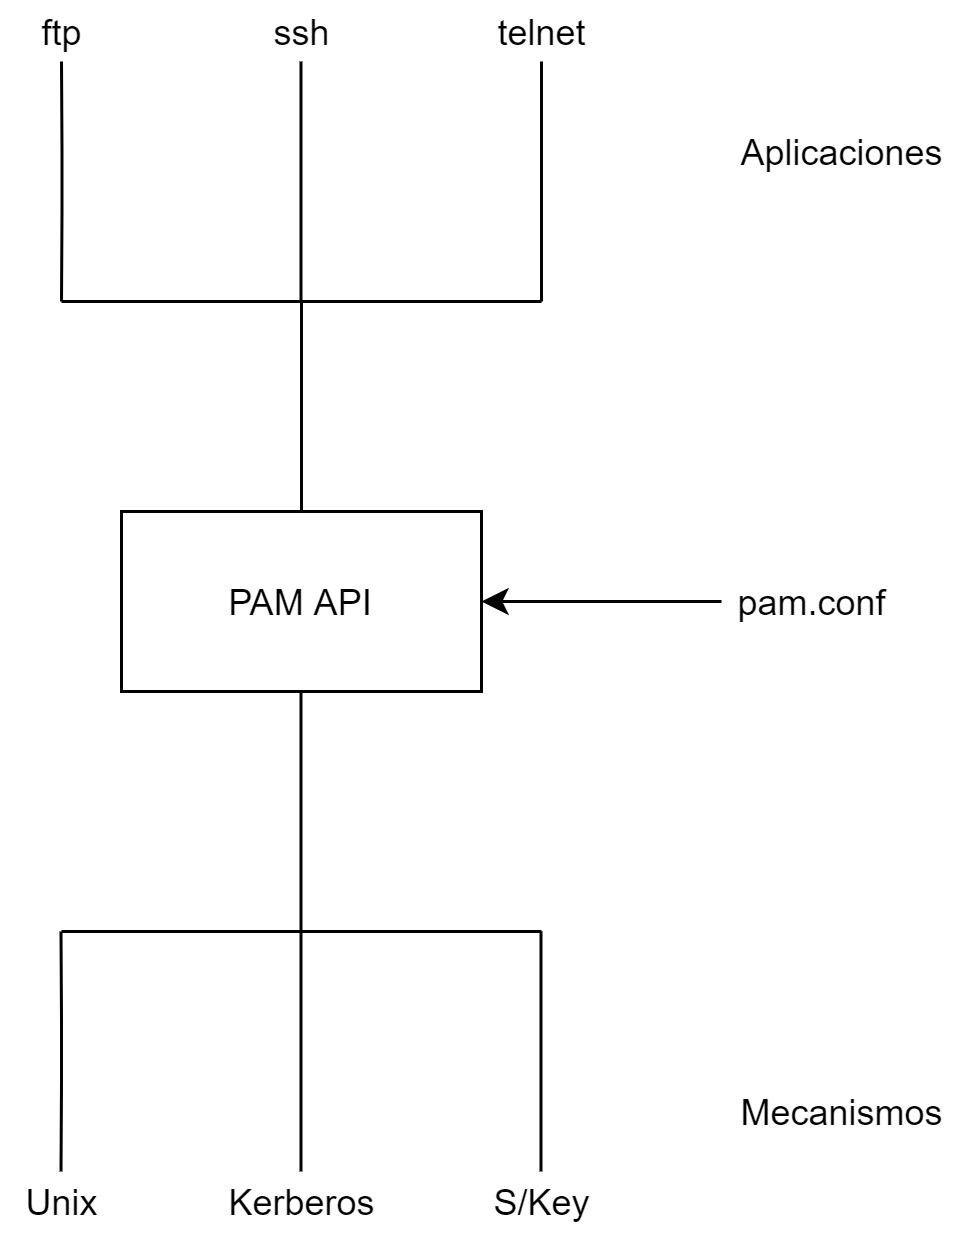
\includegraphics[scale=0.15]{pam_conf.png}
    \caption{Arquitectura básica PAM}
\end{figure}

PAM unifica autenticación y control de acceso al sistema, y permite añadir módulos de autenticación a través de interfaces bien 
definidas. Configuración en la autenticación es un componente junto a administración de cuenta, sesión y contraseñas. Para este 
trabajo, solo se va a usar la parte de autenticación ya que el resto no es necesaria. Cada una de estas áreas funcionales trabajan 
como módulos separados.

Dado la extensión y temática del trabajo, no se pretende dar detalles acerca del funcionamiento de la API de PAM. Simplemente 
anotar que para el desarrollo de este proyecto se usó las siguientes funciones de la API:

\begin{itemize}
    \item \textit{pam\_authenticate()} \cite{pam_sm_authenticate3}: función para autenticar a un usuario
    \item \textit{pam\_get\_user()} \cite{pam_get_user3}: función para obtener el nombre del usuario específico que intenta autenticarse
\end{itemize}

El archivo de configuración PAM (\textit{pam.conf}) es la base de gestión de los módulos. Tal y como se ha mencionado antes, 
cuando una aplicación solicita autenticarse usando algún mecanismo que funcione con PAM, la API comprueba los módulos a ejecutar
en este archivo así como la política que siguen.

El archivo de configuración \ref{code:pam_conf} se ha usado en el broker MQTT de este trabajo. Define los siguientes parámetros 
\cite{mosquittoconf_2021}:

\begin{itemize}
    \item \textit{log\_dest}: ruta absoluta del archivo de logs
    \item \textit{log\_type}: tipo de mensajes a registrar
    \item \textit{log\_timestamp}: añadir valor de marca de tiempo
    \item \textit{include\_dir}: ruta absoluta del directorio de archivos de configuración externos
    \item \textit{listener}: puerto de escucha
    \item \textit{cafile}: ruta absoluta del certificado de la \acf[first-style=short]{ca}
    \item \textit{certfile}: ruta absoluta del certificado del broker MQTT
    \item \textit{keyfile}: ruta absoluta de la clave privada del broker MQTT
    \item \textit{allow\_anonymous}: permitir que clientes se puedan conectar sin proporcionar claves (usuario)
\end{itemize}

El cliente \textit{mosquitto} escucha por defecto por el puerto 1883 para comunicaciones no seguras
y por el 8883 para seguras. El primero solo se usa para comunicaciones internas (\textit{localhost}).

La \acf[first-style=short]{ca} es una entidad que administra certificados digitales, los cuales son usados para vincular una entidad a una 
clave pública. Para el presente tranajo, a diferencia de \cite{multipauthpaper}, se ha usado el broker MQTT como \acf[first-style=short]{ca}. 
No obstante, la \acf[first-style=short]{ca} debe correr en un servidor independiente debido a su papel fundamental en la seguridad de toda
infraestructura y para facilitar la gestión de nodos que se incorporen a la arquitectura del sistema así como revocar aquellos
certificados de clientes que no tengan más acceso.

\section{Análisis de herramientas}
\label{sec:analisis-herramientas}

Para el presente trabajo se ha desarrollado el software usando el lenguaje de programación C dada la facilidad y documentación
disponible a la hora de desarrollar módulos PAM en dicho lenguaje. 
Se ha usado \textit{mosquitto} \cite{eclipse_2018} como cliente MQTT dado su extensa documentación, por ser un software de código 
abierto y estar escrito en C.
Con respecto al entorno de pruebas, se ha usado Vagrant \cite{vagrant} como orquestador de máquinas virtuales para desplegar el 
entorno de prueba.
